\usepackage{tikz}
\newcommand{\svcourse}{CST Part IA: Introduction to Probability}
\newcommand{\svnumber}{1}
\newcommand{\svvenue}{Churchill, Room TBD}
\newcommand{\svdate}{2022-05-14}
\newcommand{\svtime}{11:00}
\newcommand{\svuploadkey}{PO5ogKIM8KQA22FZS8IAf8gxA8XKi19jxIBVHIfFZ+3GCBXuNUXS9lVN6bNYjxM/}

\newcommand{\svrname}{Mr Matthew Ireland}
\newcommand{\jkfside}{twoside}
\newcommand{\jkfhanded}{right}

\newcommand{\studentname}{Harry Langford}
\newcommand{\studentemail}{hjel2@cam.ac.uk}


\documentclass[10pt,\jkfside,a4paper]{article}

\input{../../template/includes.tex}
% DO NOT add \usepackage commands here.  Place any custom commands
% into your SV work files.  Anything in the template directory is
% likely to be overwritten!

\usepackage{fancyhdr}

\usepackage{lastpage}       % ``n of m'' page numbering
\usepackage{lscape}         % Makes landscape easier

\usepackage{verbatim}       % Verbatim blocks
\usepackage{epsfig}         % Embed encapsulated postscript
\usepackage{array}          % Array environment
\usepackage[nolinks]{qrcode}         % QR codes
\usepackage{enumitem}       % Required by Tom Johnson's exam question header

\usepackage{hhline}         % Horizontal lines in tables
\usepackage{siunitx}        % Correct spacing of units
\usepackage{amsmath}        % American Mathematical Society
\usepackage{amssymb}        % Maths symbols
\usepackage{amsthm}         % Theorems

\usepackage{ifthen}         % Conditional processing in tex

\usepackage[top=3cm,
            bottom=3cm,
            inner=2cm,
            outer=5cm]{geometry}

% PDF metadata + URL formatting
\usepackage[
            pdfauthor={\studentname},
            pdftitle={\svcourse, SV \svnumber},
            pdfsubject={},
            pdfkeywords={9d2547b00aba40b58fa0378774f72ee6},
            pdfproducer={},
            pdfcreator={},
            hidelinks]{hyperref}

\renewcommand{\headrulewidth}{0.4pt}
\renewcommand{\footrulewidth}{0.4pt}
\fancyheadoffset[LO,LE,RO,RE]{0pt}
\fancyfootoffset[LO,LE,RO,RE]{0pt}
\pagestyle{fancy}
\fancyhead{}
\fancyhead[LO,RE]{{\bfseries \studentname}\\\studentemail}
\fancyhead[RO,LE]{{\bfseries \svcourse, SV~\svnumber}\\\svdate\ \svtime, \svvenue}
\fancyfoot{}
\fancyfoot[LO,RE]{For: \svrname}
\fancyfoot[RO,LE]{\today\hspace{1cm}\thepage\ / \pageref{LastPage}}
\fancyfoot[C]{\qrcode[height=0.8cm]{\svuploadkey}}
\setlength{\headheight}{22.55pt}

\ifthenelse{\equal{\jkfside}{oneside}}{

 \ifthenelse{\equal{\jkfhanded}{left}}{
  % 1. Left-handed marker, one-sided printing or e-marking, use oneside and...
  \evensidemargin=\oddsidemargin
  \oddsidemargin=73pt
  \setlength{\marginparwidth}{111pt}
  \setlength{\marginparsep}{-\marginparsep}
  \addtolength{\marginparsep}{-\textwidth}
  \addtolength{\marginparsep}{-\marginparwidth}
 }{
  % 2. Right-handed marker, one-sided printing or e-marking, use oneside.
  \setlength{\marginparwidth}{111pt}
 }

}{
 % 3. Alternating margins, two-sided printing, use twoside.
}

\setlength{\parindent}{0em}
\addtolength{\parskip}{1ex}

% Exam question headings, labels and sensible layout (courtesy of Tom Johnson)
\setlist{parsep=\parskip, listparindent=\parindent}
\newcommand{\examhead}[3]{\section{#1 Paper #2 Question #3}}
\newenvironment{examquestion}[3]{
    \examhead{#1}{#2}{#3}\setlist[enumerate, 1]{label=(\alph*)}\setlist[enumerate, 2]{label=(\roman*)}
    \marginpar{\qrcode{https://www.cl.cam.ac.uk/teaching/exams/pastpapers/y#1p#2q#3.pdf}}
    \marginpar{\footnotesize \url{https://www.cl.cam.ac.uk/teaching/exams/pastpapers/y#1p#2q#3.pdf}}
}{}



\usepackage{tikz}

\begin{document}

\begin{enumerate}

\item Without dwelling on the structure of the nodes and on the positional relationship between keys 
and subtrees (for which an example picture will be sufficient), give an otherwise complete and concise 
definition of a B-tree of minimum degree t, listing all the defining structural properties.

The features of a B-Tree with minimum degree $t$ are as follows:

\begin{itemize}

\item Any node has no fewer than $t - 1$ elements (with the exception of the root when the whole tree has 
fewer than $t - 1$ elements.

\item No node has more than $2t - 1$ elements.

\item A node with $n$ elements should have $n + 1$ children.

\item Every route from any node to a leaf passes through the same number of nodes.

\item Insertion into a B-Tree is done at a leaf.

\item When inserting an element into a B-Tree you should split any nodes you pass through which have $2t - 1$ 
elements.

\item When deleting an element from a B-Tree you should fill any nodes you pass through so that they have at least 
$t$ elements.

\end{itemize}

\begin{center}
\begin{tikzpicture}
\filldraw[draw=black, fill=lightgray!10] (0.6, -2) rectangle (2.3000000000000003, -1.5);
\node[anchor=center] at (0.95, -1.75) {$A$};
\node[anchor=center] at (1.45, -1.75) {$B$};
\node[anchor=center] at (1.95, -1.75) {$C$};
\filldraw[draw=black, fill=lightgray!10] (2.45, -2) rectangle (3.6500000000000004, -1.5);
\node[anchor=center] at (2.8000000000000003, -1.75) {$E$};
\node[anchor=center] at (3.3000000000000003, -1.75) {$F$};
\filldraw[draw=black, fill=lightgray!10] (3.8000000000000003, -2) rectangle (6.0, -1.5);
\node[anchor=center] at (4.15, -1.75) {$H$};
\node[anchor=center] at (4.65, -1.75) {$I$};
\node[anchor=center] at (5.15, -1.75) {$J$};
\node[anchor=center] at (5.65, -1.75) {$K$};
\filldraw[draw=black, fill=lightgray!10] (2.6999999999999997, -1) rectangle (3.9, -0.5);
\draw [-stealth] (2.8, -0.9) -- (1.4500000000000002, -1.5);
\draw [-stealth] (3.3, -0.9) -- (3.05, -1.5);
\draw [-stealth] (3.8, -0.9) -- (4.9, -1.5);
\node[anchor=center] at (3.05, -0.75) {$D$};
\node[anchor=center] at (3.55, -0.75) {$G$};
\filldraw[draw=black, fill=lightgray!10] (6.5, -2) rectangle (7.699999999999999, -1.5);
\node[anchor=center] at (6.85, -1.75) {$M$};
\node[anchor=center] at (7.35, -1.75) {$N$};
\filldraw[draw=black, fill=lightgray!10] (7.85, -2) rectangle (10.049999999999999, -1.5);
\node[anchor=center] at (8.2, -1.75) {$P$};
\node[anchor=center] at (8.7, -1.75) {$Q$};
\node[anchor=center] at (9.2, -1.75) {$R$};
\node[anchor=center] at (9.7, -1.75) {$S$};
\filldraw[draw=black, fill=lightgray!10] (10.2, -2) rectangle (11.899999999999999, -1.5);
\node[anchor=center] at (10.549999999999999, -1.75) {$U$};
\node[anchor=center] at (11.049999999999999, -1.75) {$V$};
\node[anchor=center] at (11.549999999999999, -1.75) {$W$};
\filldraw[draw=black, fill=lightgray!10] (12.049999999999999, -2) rectangle (13.249999999999998, -1.5);
\node[anchor=center] at (12.399999999999999, -1.75) {$Y$};
\node[anchor=center] at (12.899999999999999, -1.75) {$Z$};
\filldraw[draw=black, fill=lightgray!10] (9.025, -1) rectangle (10.725, -0.5);
\draw [-stealth] (9.125, -0.9) -- (7.1, -1.5);
\draw [-stealth] (9.625, -0.9) -- (8.95, -1.5);
\draw [-stealth] (10.125, -0.9) -- (11.05, -1.5);
\draw [-stealth] (10.625, -0.9) -- (12.649999999999999, -1.5);
\node[anchor=center] at (9.375, -0.75) {$O$};
\node[anchor=center] at (9.875, -0.75) {$T$};
\node[anchor=center] at (10.375, -0.75) {$X$};
\filldraw[draw=black, fill=lightgray!10] (6.574999999999999, 0) rectangle (7.274999999999999, 0.5);
\draw [-stealth] (6.674999999999999, 0.1) -- (3.3000000000000003, -0.5);
\draw [-stealth] (7.174999999999999, 0.1) -- (9.874999999999998, -0.5);
\node[anchor=center] at (6.924999999999999, 0.25) {$L$};
\end{tikzpicture}
\end{center}

\item Explain how to insert a new item into a B-tree, showing that the algorithm preserves the B-tree 
properties you gave above.
Then insert the following values, in this order, into an initially empty
B-tree whose nodes hold at most three keys each: C A M B R I D G E X. Produce a frame-by-frame ``movie'' 
in which you redraw the tree whenever it changes in any way.

The first three insertions ($C$, $A$, $M$) are simple -- we do not reach the largest node size and so simply insert them 
into the root node without any issues.

\begin{center}
\begin{tikzpicture}
\filldraw[draw=black, fill=lightgray!10] (-0.1, 0) rectangle (1.6, 0.5);
\node[anchor=center] at (0.25, 0.25) {$A$};
\node[anchor=center] at (0.75, 0.25) {$C$};
\node[anchor=center] at (1.25, 0.25) {$M$};
\end{tikzpicture}
\end{center}

Inserting $B$ is more problematic.
The root node is full.
So when we reach the root node, we split it, promoting
the middle element ($C$) to the new root node and placing the other two elements in new nodes -- each the children 
of $C$.
Now we insert $B$ without issue, seeing it is less than $C$ but greater than $A$ so insert it to the right of $A$.

\begin{center}
\begin{tikzpicture}
\filldraw[draw=black, fill=lightgray!10] (0.24999999999999997, -1) rectangle (1.4500000000000002, -0.5);
\node[anchor=center] at (0.6, -0.75) {$A$};
\node[anchor=center] at (1.1, -0.75) {$B$};
\filldraw[draw=black, fill=lightgray!10] (1.6, -1) rectangle (2.3000000000000003, -0.5);
\node[anchor=center] at (1.9500000000000002, -0.75) {$M$};
\filldraw[draw=black, fill=lightgray!10] (0.9250000000000002, 0) rectangle (1.6250000000000002, 0.5);
\draw [-stealth] (1.0250000000000001, 0.1) -- (0.8500000000000001, -0.5);
\draw [-stealth] (1.5250000000000001, 0.1) -- (1.9500000000000002, -0.5);
\node[anchor=center] at (1.2750000000000001, 0.25) {$C$};
\end{tikzpicture}
\end{center}

We insert $I$ and $R$ without having to take any action to preserve the properties of the B-Tree. These insertions are 
simple traversal.

\begin{center}
\begin{tikzpicture}
\filldraw[draw=black, fill=lightgray!10] (0.24999999999999997, -1) rectangle (1.4500000000000002, -0.5);
\node[anchor=center] at (0.6, -0.75) {$A$};
\node[anchor=center] at (1.1, -0.75) {$B$};
\filldraw[draw=black, fill=lightgray!10] (1.6, -1) rectangle (3.3000000000000003, -0.5);
\node[anchor=center] at (1.9500000000000002, -0.75) {$I$};
\node[anchor=center] at (2.45, -0.75) {$M$};
\node[anchor=center] at (2.95, -0.75) {$R$};
\filldraw[draw=black, fill=lightgray!10] (1.425, 0) rectangle (2.1250000000000004, 0.5);
\draw [-stealth] (1.5250000000000001, 0.1) -- (0.8500000000000001, -0.5);
\draw [-stealth] (2.0250000000000004, 0.1) -- (2.45, -0.5);
\node[anchor=center] at (1.7750000000000001, 0.25) {$C$};
\end{tikzpicture}
\end{center}

When we insert $D$, we notice that the node containing $I$, $M$, $R$ is full, and so split it, promoting the 
middle element $M$ into the parent node. We then insert $D$ into the correct child node.

\begin{center}
\begin{tikzpicture}
\filldraw[draw=black, fill=lightgray!10] (0.24999999999999997, -1) rectangle (1.4500000000000002, -0.5);
\node[anchor=center] at (0.6, -0.75) {$A$};
\node[anchor=center] at (1.1, -0.75) {$B$};
\filldraw[draw=black, fill=lightgray!10] (1.6, -1) rectangle (2.8000000000000003, -0.5);
\node[anchor=center] at (1.9500000000000002, -0.75) {$D$};
\node[anchor=center] at (2.45, -0.75) {$I$};
\filldraw[draw=black, fill=lightgray!10] (2.95, -1) rectangle (3.6500000000000004, -0.5);
\node[anchor=center] at (3.3000000000000003, -0.75) {$R$};
\filldraw[draw=black, fill=lightgray!10] (1.35, 0) rectangle (2.5500000000000003, 0.5);
\draw [-stealth] (1.4500000000000002, 0.1) -- (0.8500000000000001, -0.5);
\draw [-stealth] (1.9500000000000002, 0.1) -- (2.2, -0.5);
\draw [-stealth] (2.45, 0.1) -- (3.3, -0.5);
\node[anchor=center] at (1.7000000000000002, 0.25) {$C$};
\node[anchor=center] at (2.2, 0.25) {$M$};
\end{tikzpicture}
\end{center}

$G$ is inserted in a simple traversal.

\begin{center}
\begin{tikzpicture}
\filldraw[draw=black, fill=lightgray!10] (0.24999999999999997, -1) rectangle (1.4500000000000002, -0.5);
\node[anchor=center] at (0.6, -0.75) {$A$};
\node[anchor=center] at (1.1, -0.75) {$B$};
\filldraw[draw=black, fill=lightgray!10] (1.6, -1) rectangle (3.3000000000000003, -0.5);
\node[anchor=center] at (1.9500000000000002, -0.75) {$D$};
\node[anchor=center] at (2.45, -0.75) {$G$};
\node[anchor=center] at (2.95, -0.75) {$I$};
\filldraw[draw=black, fill=lightgray!10] (3.45, -1) rectangle (4.15, -0.5);
\node[anchor=center] at (3.8000000000000003, -0.75) {$R$};
\filldraw[draw=black, fill=lightgray!10] (1.6, 0) rectangle (2.8000000000000003, 0.5);
\draw [-stealth] (1.7000000000000002, 0.1) -- (0.8500000000000001, -0.5);
\draw [-stealth] (2.2, 0.1) -- (2.45, -0.5);
\draw [-stealth] (2.7, 0.1) -- (3.8000000000000003, -0.5);
\node[anchor=center] at (1.9500000000000002, 0.25) {$C$};
\node[anchor=center] at (2.45, 0.25) {$M$};
\end{tikzpicture}
\end{center}

when inserting $E$, we reach the node $D$, $G$, $I$ -- which is full. So we must split this node, promoting the 
middle node into the parent node.

\begin{center}
\begin{tikzpicture}
\filldraw[draw=black, fill=lightgray!10] (0.24999999999999997, -1) rectangle (1.4500000000000002, -0.5);
\node[anchor=center] at (0.6, -0.75) {$A$};
\node[anchor=center] at (1.1, -0.75) {$B$};
\filldraw[draw=black, fill=lightgray!10] (1.6, -1) rectangle (2.8000000000000003, -0.5);
\node[anchor=center] at (1.9500000000000002, -0.75) {$D$};
\node[anchor=center] at (2.45, -0.75) {$E$};
\filldraw[draw=black, fill=lightgray!10] (2.95, -1) rectangle (3.6500000000000004, -0.5);
\node[anchor=center] at (3.3000000000000003, -0.75) {$I$};
\filldraw[draw=black, fill=lightgray!10] (3.8000000000000003, -1) rectangle (4.5, -0.5);
\node[anchor=center] at (4.15, -0.75) {$R$};
\filldraw[draw=black, fill=lightgray!10] (1.525, 0) rectangle (3.225, 0.5);
\draw [-stealth] (1.625, 0.1) -- (0.8500000000000001, -0.5);
\draw [-stealth] (2.125, 0.1) -- (2.2, -0.5);
\draw [-stealth] (2.625, 0.1) -- (3.3, -0.5);
\draw [-stealth] (3.125, 0.1) -- (4.15, -0.5);
\node[anchor=center] at (1.875, 0.25) {$C$};
\node[anchor=center] at (2.375, 0.25) {$G$};
\node[anchor=center] at (2.875, 0.25) {$M$};
\end{tikzpicture}
\end{center}

The next insertion finds that the root is full and so splits in, promoting the middle element $G$ to the 
new root node. We then insert $X$ in a trivial insertion.

\begin{center}
\begin{tikzpicture}
\filldraw[draw=black, fill=lightgray!10] (0.6, -2) rectangle (1.8, -1.5);
\node[anchor=center] at (0.95, -1.75) {$A$};
\node[anchor=center] at (1.45, -1.75) {$B$};
\filldraw[draw=black, fill=lightgray!10] (1.9499999999999997, -2) rectangle (3.15, -1.5);
\node[anchor=center] at (2.3, -1.75) {$D$};
\node[anchor=center] at (2.8, -1.75) {$E$};
\filldraw[draw=black, fill=lightgray!10] (1.525, -1) rectangle (2.225, -0.5);
\draw [-stealth] (1.625, -0.9) -- (1.2, -1.5);
\draw [-stealth] (2.125, -0.9) -- (2.55, -1.5);
\node[anchor=center] at (1.875, -0.75) {$C$};
\filldraw[draw=black, fill=lightgray!10] (3.65, -2) rectangle (4.35, -1.5);
\node[anchor=center] at (4.0, -1.75) {$I$};
\filldraw[draw=black, fill=lightgray!10] (4.5, -2) rectangle (5.699999999999999, -1.5);
\node[anchor=center] at (4.85, -1.75) {$R$};
\node[anchor=center] at (5.35, -1.75) {$X$};
\filldraw[draw=black, fill=lightgray!10] (4.325, -1) rectangle (5.0249999999999995, -0.5);
\draw [-stealth] (4.425, -0.9) -- (4.0, -1.5);
\draw [-stealth] (4.925, -0.9) -- (5.1, -1.5);
\node[anchor=center] at (4.675, -0.75) {$M$};
\filldraw[draw=black, fill=lightgray!10] (2.8, 0) rectangle (3.5, 0.5);
\draw [-stealth] (2.9, 0.1) -- (1.875, -0.5);
\draw [-stealth] (3.4, 0.1) -- (4.674999999999999, -0.5);
\node[anchor=center] at (3.15, 0.25) {$G$};
\end{tikzpicture}
\end{center}


\item Explain how to delete a value from a B-tree and illustrate your algorithm by showing frame-by-frame
 movies for the deletion of M, Q, Y, in that order, from the following B-tree. As before, each node holds 
 at most three keys.

\begin{center}
\begin{tikzpicture}
\filldraw[draw=black, fill=lightgray!10] (0.6, -2) rectangle (1.8, -1.5);
\node[anchor=center] at (0.95, -1.75) {$A$};
\node[anchor=center] at (1.45, -1.75) {$B$};
\filldraw[draw=black, fill=lightgray!10] (1.9499999999999997, -2) rectangle (3.65, -1.5);
\node[anchor=center] at (2.3, -1.75) {$D$};
\node[anchor=center] at (2.8, -1.75) {$E$};
\node[anchor=center] at (3.3, -1.75) {$F$};
\filldraw[draw=black, fill=lightgray!10] (3.8, -2) rectangle (5.0, -1.5);
\node[anchor=center] at (4.15, -1.75) {$H$};
\node[anchor=center] at (4.65, -1.75) {$I$};
\filldraw[draw=black, fill=lightgray!10] (2.1999999999999997, -1) rectangle (3.4, -0.5);
\draw [-stealth] (2.3, -0.9) -- (1.2, -1.5);
\draw [-stealth] (2.8, -0.9) -- (2.8, -1.5);
\draw [-stealth] (3.3, -0.9) -- (4.3999999999999995, -1.5);
\node[anchor=center] at (2.55, -0.75) {$C$};
\node[anchor=center] at (3.05, -0.75) {$G$};
\filldraw[draw=black, fill=lightgray!10] (5.5, -2) rectangle (6.699999999999999, -1.5);
\node[anchor=center] at (5.85, -1.75) {$K$};
\node[anchor=center] at (6.35, -1.75) {$L$};
\filldraw[draw=black, fill=lightgray!10] (6.85, -2) rectangle (8.549999999999999, -1.5);
\node[anchor=center] at (7.199999999999999, -1.75) {$N$};
\node[anchor=center] at (7.699999999999999, -1.75) {$O$};
\node[anchor=center] at (8.2, -1.75) {$P$};
\filldraw[draw=black, fill=lightgray!10] (8.7, -2) rectangle (9.399999999999999, -1.5);
\node[anchor=center] at (9.049999999999999, -1.75) {$R$};
\filldraw[draw=black, fill=lightgray!10] (9.549999999999999, -2) rectangle (10.249999999999998, -1.5);
\node[anchor=center] at (9.899999999999999, -1.75) {$U$};
\filldraw[draw=black, fill=lightgray!10] (7.0249999999999995, -1) rectangle (8.725, -0.5);
\draw [-stealth] (7.124999999999999, -0.9) -- (6.1, -1.5);
\draw [-stealth] (7.624999999999999, -0.9) -- (7.699999999999999, -1.5);
\draw [-stealth] (8.125, -0.9) -- (9.05, -1.5);
\draw [-stealth] (8.625, -0.9) -- (9.899999999999999, -1.5);
\node[anchor=center] at (7.374999999999999, -0.75) {$M$};
\node[anchor=center] at (7.874999999999999, -0.75) {$Q$};
\node[anchor=center] at (8.375, -0.75) {$T$};
\filldraw[draw=black, fill=lightgray!10] (10.749999999999998, -2) rectangle (11.449999999999998, -1.5);
\node[anchor=center] at (11.099999999999998, -1.75) {$X$};
\filldraw[draw=black, fill=lightgray!10] (11.599999999999998, -2) rectangle (12.299999999999997, -1.5);
\node[anchor=center] at (11.949999999999998, -1.75) {$Z$};
\filldraw[draw=black, fill=lightgray!10] (11.174999999999999, -1) rectangle (11.874999999999998, -0.5);
\draw [-stealth] (11.274999999999999, -0.9) -- (11.099999999999998, -1.5);
\draw [-stealth] (11.774999999999999, -0.9) -- (11.95, -1.5);
\node[anchor=center] at (11.524999999999999, -0.75) {$Y$};
\filldraw[draw=black, fill=lightgray!10] (5.849999999999999, 0) rectangle (7.049999999999998, 0.5);
\draw [-stealth] (5.949999999999998, 0.1) -- (2.8000000000000003, -0.5);
\draw [-stealth] (6.449999999999998, 0.1) -- (7.874999999999999, -0.5);
\draw [-stealth] (6.949999999999998, 0.1) -- (11.524999999999997, -0.5);
\node[anchor=center] at (6.199999999999998, 0.25) {$J$};
\node[anchor=center] at (6.699999999999998, 0.25) {$V$};
\end{tikzpicture}
\end{center}

Since $M$ is an internal node, we cannot delete $M$ without manipulating the tree slightly. Since the successor of 
$M$ ($N$) is in a node which is not of the minimum degree, we can replace $M$ with it's successor and then delete 
the successor without further manipulation. The tree after this has happened is shown below with the affected nodes 
highlighted.

\begin{center}
\begin{tikzpicture}
\filldraw[draw=black, fill=lightgray!10] (0.6, -2) rectangle (1.8, -1.5);
\node[anchor=center] at (0.95, -1.75) {$A$};
\node[anchor=center] at (1.45, -1.75) {$B$};
\filldraw[draw=black, fill=lightgray!10] (1.9499999999999997, -2) rectangle (3.65, -1.5);
\node[anchor=center] at (2.3, -1.75) {$D$};
\node[anchor=center] at (2.8, -1.75) {$E$};
\node[anchor=center] at (3.3, -1.75) {$F$};
\filldraw[draw=black, fill=lightgray!10] (3.8, -2) rectangle (5.0, -1.5);
\node[anchor=center] at (4.15, -1.75) {$H$};
\node[anchor=center] at (4.65, -1.75) {$I$};
\filldraw[draw=black, fill=lightgray!10] (2.1999999999999997, -1) rectangle (3.4, -0.5);
\draw [-stealth] (2.3, -0.9) -- (1.2, -1.5);
\draw [-stealth] (2.8, -0.9) -- (2.8, -1.5);
\draw [-stealth] (3.3, -0.9) -- (4.3999999999999995, -1.5);
\node[anchor=center] at (2.55, -0.75) {$C$};
\node[anchor=center] at (3.05, -0.75) {$G$};
\filldraw[draw=black, fill=lightgray!10] (5.5, -2) rectangle (6.699999999999999, -1.5);
\node[anchor=center] at (5.85, -1.75) {$K$};
\node[anchor=center] at (6.35, -1.75) {$L$};
\filldraw[draw=black, fill=red!10] (6.85, -2) rectangle (8.049999999999999, -1.5);
\node[anchor=center] at (7.199999999999999, -1.75) {$O$};
\node[anchor=center] at (7.699999999999999, -1.75) {$P$};
\filldraw[draw=black, fill=lightgray!10] (8.2, -2) rectangle (8.899999999999999, -1.5);
\node[anchor=center] at (8.549999999999999, -1.75) {$R$};
\filldraw[draw=black, fill=lightgray!10] (9.049999999999999, -2) rectangle (9.749999999999998, -1.5);
\node[anchor=center] at (9.399999999999999, -1.75) {$U$};
\filldraw[draw=black, fill=red!10] (6.7749999999999995, -1) rectangle (8.475, -0.5);
\draw [-stealth] (6.874999999999999, -0.9) -- (6.1, -1.5);
\draw [-stealth] (7.374999999999999, -0.9) -- (7.449999999999999, -1.5);
\draw [-stealth] (7.874999999999999, -0.9) -- (8.55, -1.5);
\draw [-stealth] (8.375, -0.9) -- (9.399999999999999, -1.5);
\node[anchor=center] at (7.124999999999999, -0.75) {$N$};
\node[anchor=center] at (7.624999999999999, -0.75) {$Q$};
\node[anchor=center] at (8.125, -0.75) {$T$};
\filldraw[draw=black, fill=lightgray!10] (10.249999999999998, -2) rectangle (10.949999999999998, -1.5);
\node[anchor=center] at (10.599999999999998, -1.75) {$X$};
\filldraw[draw=black, fill=lightgray!10] (11.099999999999998, -2) rectangle (11.799999999999997, -1.5);
\node[anchor=center] at (11.449999999999998, -1.75) {$Z$};
\filldraw[draw=black, fill=lightgray!10] (10.674999999999999, -1) rectangle (11.374999999999998, -0.5);
\draw [-stealth] (10.774999999999999, -0.9) -- (10.599999999999998, -1.5);
\draw [-stealth] (11.274999999999999, -0.9) -- (11.45, -1.5);
\node[anchor=center] at (11.024999999999999, -0.75) {$Y$};
\filldraw[draw=black, fill=lightgray!10] (5.599999999999999, 0) rectangle (6.799999999999998, 0.5);
\draw [-stealth] (5.699999999999998, 0.1) -- (2.8000000000000003, -0.5);
\draw [-stealth] (6.199999999999998, 0.1) -- (7.624999999999999, -0.5);
\draw [-stealth] (6.699999999999998, 0.1) -- (11.024999999999997, -0.5);
\node[anchor=center] at (5.949999999999998, 0.25) {$J$};
\node[anchor=center] at (6.449999999999998, 0.25) {$V$};
\end{tikzpicture}
\end{center}

To delete $Q$ we notice that the successor ($R$) is in a node of minimum degree -- so we cannot replace $Q$ with $R$. 
Next we check the predecessor -- in this case $P$. We notice that $P$ is in a node which is not of the minimum 
degree and so we can replace $Q$ with $P$ and then delete $P$ from the node it was in while still satisfying all 
the B-Tree properties.

\begin{center}
\begin{tikzpicture}
\filldraw[draw=black, fill=lightgray!10] (0.6, -2) rectangle (1.8, -1.5);
\node[anchor=center] at (0.95, -1.75) {$A$};
\node[anchor=center] at (1.45, -1.75) {$B$};
\filldraw[draw=black, fill=lightgray!10] (1.9499999999999997, -2) rectangle (3.65, -1.5);
\node[anchor=center] at (2.3, -1.75) {$D$};
\node[anchor=center] at (2.8, -1.75) {$E$};
\node[anchor=center] at (3.3, -1.75) {$F$};
\filldraw[draw=black, fill=lightgray!10] (3.8, -2) rectangle (5.0, -1.5);
\node[anchor=center] at (4.15, -1.75) {$H$};
\node[anchor=center] at (4.65, -1.75) {$I$};
\filldraw[draw=black, fill=lightgray!10] (2.1999999999999997, -1) rectangle (3.4, -0.5);
\draw [-stealth] (2.3, -0.9) -- (1.2, -1.5);
\draw [-stealth] (2.8, -0.9) -- (2.8, -1.5);
\draw [-stealth] (3.3, -0.9) -- (4.3999999999999995, -1.5);
\node[anchor=center] at (2.55, -0.75) {$C$};
\node[anchor=center] at (3.05, -0.75) {$G$};
\filldraw[draw=black, fill=lightgray!10] (5.5, -2) rectangle (6.699999999999999, -1.5);
\node[anchor=center] at (5.85, -1.75) {$K$};
\node[anchor=center] at (6.35, -1.75) {$L$};
\filldraw[draw=black, fill=red!10] (6.85, -2) rectangle (7.549999999999999, -1.5);
\node[anchor=center] at (7.199999999999999, -1.75) {$O$};
\filldraw[draw=black, fill=lightgray!10] (7.699999999999999, -2) rectangle (8.399999999999999, -1.5);
\node[anchor=center] at (8.049999999999999, -1.75) {$R$};
\filldraw[draw=black, fill=lightgray!10] (8.549999999999999, -2) rectangle (9.249999999999998, -1.5);
\node[anchor=center] at (8.899999999999999, -1.75) {$U$};
\filldraw[draw=black, fill=red!10] (6.5249999999999995, -1) rectangle (8.225, -0.5);
\draw [-stealth] (6.624999999999999, -0.9) -- (6.1, -1.5);
\draw [-stealth] (7.124999999999999, -0.9) -- (7.199999999999999, -1.5);
\draw [-stealth] (7.624999999999999, -0.9) -- (8.049999999999999, -1.5);
\draw [-stealth] (8.125, -0.9) -- (8.899999999999999, -1.5);
\node[anchor=center] at (6.874999999999999, -0.75) {$N$};
\node[anchor=center] at (7.374999999999999, -0.75) {$P$};
\node[anchor=center] at (7.874999999999999, -0.75) {$T$};
\filldraw[draw=black, fill=lightgray!10] (9.749999999999998, -2) rectangle (10.449999999999998, -1.5);
\node[anchor=center] at (10.099999999999998, -1.75) {$X$};
\filldraw[draw=black, fill=lightgray!10] (10.599999999999998, -2) rectangle (11.299999999999997, -1.5);
\node[anchor=center] at (10.949999999999998, -1.75) {$Z$};
\filldraw[draw=black, fill=lightgray!10] (10.174999999999999, -1) rectangle (10.874999999999998, -0.5);
\draw [-stealth] (10.274999999999999, -0.9) -- (10.099999999999998, -1.5);
\draw [-stealth] (10.774999999999999, -0.9) -- (10.95, -1.5);
\node[anchor=center] at (10.524999999999999, -0.75) {$Y$};
\filldraw[draw=black, fill=lightgray!10] (5.349999999999999, 0) rectangle (6.549999999999998, 0.5);
\draw [-stealth] (5.449999999999998, 0.1) -- (2.8000000000000003, -0.5);
\draw [-stealth] (5.949999999999998, 0.1) -- (7.374999999999999, -0.5);
\draw [-stealth] (6.449999999999998, 0.1) -- (10.524999999999997, -0.5);
\node[anchor=center] at (5.699999999999998, 0.25) {$J$};
\node[anchor=center] at (6.199999999999998, 0.25) {$V$};
\end{tikzpicture}
\end{center}

In order to delete $Y$ we notice that $Y$ is in a node of minimum degree. So we cannot delete $Y$ without violating 
the properties of a B-Tree. However, since $Y$ has a sibling -- in this case it's neighbour $N$, $P$ $T$ -- which has 
more than the minimum degree. So we can ``shuffle'' across nodes from the sibling. We do this by moving the rightmost 
element in the sibling into the parent and moving the successor down into the original node (with $Y$ in it). 
The diagram of this is shown as below. We must also move $U$ across in order to preserve the properties of the B-Tree.
Now we are deleting from a node with more than the minimum degree.

\begin{center}
\begin{tikzpicture}
\filldraw[draw=black, fill=lightgray!10] (0.6, -2) rectangle (1.8, -1.5);
\node[anchor=center] at (0.95, -1.75) {$A$};
\node[anchor=center] at (1.45, -1.75) {$B$};
\filldraw[draw=black, fill=lightgray!10] (1.9499999999999997, -2) rectangle (3.65, -1.5);
\node[anchor=center] at (2.3, -1.75) {$D$};
\node[anchor=center] at (2.8, -1.75) {$E$};
\node[anchor=center] at (3.3, -1.75) {$F$};
\filldraw[draw=black, fill=lightgray!10] (3.8, -2) rectangle (5.0, -1.5);
\node[anchor=center] at (4.15, -1.75) {$H$};
\node[anchor=center] at (4.65, -1.75) {$I$};
\filldraw[draw=black, fill=lightgray!10] (2.1999999999999997, -1) rectangle (3.4, -0.5);
\draw [-stealth] (2.3, -0.9) -- (1.2, -1.5);
\draw [-stealth] (2.8, -0.9) -- (2.8, -1.5);
\draw [-stealth] (3.3, -0.9) -- (4.3999999999999995, -1.5);
\node[anchor=center] at (2.55, -0.75) {$C$};
\node[anchor=center] at (3.05, -0.75) {$G$};
\filldraw[draw=black, fill=lightgray!10] (5.5, -2) rectangle (6.699999999999999, -1.5);
\node[anchor=center] at (5.85, -1.75) {$K$};
\node[anchor=center] at (6.35, -1.75) {$L$};
\filldraw[draw=black, fill=lightgray!10] (6.85, -2) rectangle (7.549999999999999, -1.5);
\node[anchor=center] at (7.199999999999999, -1.75) {$O$};
\filldraw[draw=black, fill=lightgray!10] (7.699999999999999, -2) rectangle (8.399999999999999, -1.5);
\node[anchor=center] at (8.049999999999999, -1.75) {$R$};
\filldraw[draw=black, fill=red!10] (6.35, -1) rectangle (7.549999999999999, -0.5);
\draw [-stealth] (6.449999999999999, -0.9) -- (6.1, -1.5);
\draw [-stealth] (6.949999999999999, -0.9) -- (7.199999999999999, -1.5);
\draw [-stealth] (7.449999999999999, -0.9) -- (8.049999999999999, -1.5);
\node[anchor=center] at (6.699999999999999, -0.75) {$N$};
\node[anchor=center] at (7.199999999999999, -0.75) {$P$};
\filldraw[draw=black, fill=lightgray!10] (8.899999999999999, -2) rectangle (9.599999999999998, -1.5);
\node[anchor=center] at (9.249999999999998, -1.75) {$U$};
\filldraw[draw=black, fill=lightgray!10] (9.749999999999998, -2) rectangle (10.449999999999998, -1.5);
\node[anchor=center] at (10.099999999999998, -1.75) {$X$};
\filldraw[draw=black, fill=lightgray!10] (10.599999999999998, -2) rectangle (11.299999999999997, -1.5);
\node[anchor=center] at (10.949999999999998, -1.75) {$Z$};
\filldraw[draw=black, fill=red!10] (9.499999999999998, -1) rectangle (10.699999999999998, -0.5);
\draw [-stealth] (9.599999999999998, -0.9) -- (9.25, -1.5);
\draw [-stealth] (10.099999999999998, -0.9) -- (10.099999999999998, -1.5);
\draw [-stealth] (10.599999999999998, -0.9) -- (10.95, -1.5);
\node[anchor=center] at (9.849999999999998, -0.75) {$V$};
\node[anchor=center] at (10.349999999999998, -0.75) {$Y$};
\filldraw[draw=black, fill=red!10] (5.349999999999999, 0) rectangle (6.549999999999998, 0.5);
\draw [-stealth] (5.449999999999998, 0.1) -- (2.8000000000000003, -0.5);
\draw [-stealth] (5.949999999999998, 0.1) -- (6.949999999999999, -0.5);
\draw [-stealth] (6.449999999999998, 0.1) -- (10.099999999999998, -0.5);
\node[anchor=center] at (5.699999999999998, 0.25) {$J$};
\node[anchor=center] at (6.199999999999998, 0.25) {$T$};
\end{tikzpicture}
\end{center}

We notice both $Y$'s successor and predecessor are in nodes of minimum degree. This means we cannot promote either of them 
otherwise we would have a node with less than the minimum degree.
So we merge $Y$'s children and delete $Y$. This preserves the properties of the B-Tree.

\begin{center}
\begin{tikzpicture}
\filldraw[draw=black, fill=lightgray!10] (0.6, -2) rectangle (1.8, -1.5);
\node[anchor=center] at (0.95, -1.75) {$A$};
\node[anchor=center] at (1.45, -1.75) {$B$};
\filldraw[draw=black, fill=lightgray!10] (1.9499999999999997, -2) rectangle (3.65, -1.5);
\node[anchor=center] at (2.3, -1.75) {$D$};
\node[anchor=center] at (2.8, -1.75) {$E$};
\node[anchor=center] at (3.3, -1.75) {$F$};
\filldraw[draw=black, fill=lightgray!10] (3.8, -2) rectangle (5.0, -1.5);
\node[anchor=center] at (4.15, -1.75) {$H$};
\node[anchor=center] at (4.65, -1.75) {$I$};
\filldraw[draw=black, fill=lightgray!10] (2.1999999999999997, -1) rectangle (3.4, -0.5);
\draw [-stealth] (2.3, -0.9) -- (1.2, -1.5);
\draw [-stealth] (2.8, -0.9) -- (2.8, -1.5);
\draw [-stealth] (3.3, -0.9) -- (4.3999999999999995, -1.5);
\node[anchor=center] at (2.55, -0.75) {$C$};
\node[anchor=center] at (3.05, -0.75) {$G$};
\filldraw[draw=black, fill=lightgray!10] (5.5, -2) rectangle (6.699999999999999, -1.5);
\node[anchor=center] at (5.85, -1.75) {$K$};
\node[anchor=center] at (6.35, -1.75) {$L$};
\filldraw[draw=black, fill=lightgray!10] (6.85, -2) rectangle (7.549999999999999, -1.5);
\node[anchor=center] at (7.199999999999999, -1.75) {$O$};
\filldraw[draw=black, fill=lightgray!10] (7.699999999999999, -2) rectangle (8.399999999999999, -1.5);
\node[anchor=center] at (8.049999999999999, -1.75) {$R$};
\filldraw[draw=black, fill=lightgray!10] (6.35, -1) rectangle (7.549999999999999, -0.5);
\draw [-stealth] (6.449999999999999, -0.9) -- (6.1, -1.5);
\draw [-stealth] (6.949999999999999, -0.9) -- (7.199999999999999, -1.5);
\draw [-stealth] (7.449999999999999, -0.9) -- (8.049999999999999, -1.5);
\node[anchor=center] at (6.699999999999999, -0.75) {$N$};
\node[anchor=center] at (7.199999999999999, -0.75) {$P$};
\filldraw[draw=black, fill=lightgray!10] (8.899999999999999, -2) rectangle (9.599999999999998, -1.5);
\node[anchor=center] at (9.249999999999998, -1.75) {$U$};
\filldraw[draw=black, fill=red!10] (9.749999999999998, -2) rectangle (10.949999999999998, -1.5);
\node[anchor=center] at (10.099999999999998, -1.75) {$X$};
\node[anchor=center] at (10.599999999999998, -1.75) {$Z$};
\filldraw[draw=black, fill=red!10] (9.575, -1) rectangle (10.274999999999999, -0.5);
\draw [-stealth] (9.674999999999999, -0.9) -- (9.25, -1.5);
\draw [-stealth] (10.174999999999999, -0.9) -- (10.349999999999998, -1.5);
\node[anchor=center] at (9.924999999999999, -0.75) {$V$};
\filldraw[draw=black, fill=lightgray!10] (5.174999999999999, 0) rectangle (6.374999999999998, 0.5);
\draw [-stealth] (5.274999999999999, 0.1) -- (2.8000000000000003, -0.5);
\draw [-stealth] (5.774999999999999, 0.1) -- (6.949999999999999, -0.5);
\draw [-stealth] (6.274999999999999, 0.1) -- (9.924999999999999, -0.5);
\node[anchor=center] at (5.524999999999999, 0.25) {$J$};
\node[anchor=center] at (6.024999999999999, 0.25) {$T$};
\end{tikzpicture}
\end{center}


\item Briefly explain what a binary search tree (BST) is, listing its properties.

A binary search tree is a tree where each node has 0--2 children. Every node in the left subtree is smaller
than the parent and every node in the right subtree is greater than the parent. Duplicate 
elements are not allowed in a Binary \textit{Search} Tree.

\item Describe an optimally efficient algorithm to find the predecessor of a given node $n$ in a BST and 
explain why it works.

There are two cases:

\begin{enumerate}

\item The node $n$ has a left child.

If the node $n$ has a left child then you must traverse into the left subtree and then traverse into the right 
subtrees until you reach a node which has no right subtree. This is the predecessor to the node $n$.

If $n$ has a left child then every node to the left is less than $n$.
Let the predecessor to $n$ be $p$. Assume that the $p$ is not in the left subtree. 
Then there are three subcases:
\begin{itemize}

\item $p$ is in the right subtree of $n$. However this violates the BST property that all elements in the right 
subtree are less than the element. So $p$ cannot be in the right subtree.

\item There is some ancestor $a$ of $n$ such that $p$ is in the left subtree and $n$ is in the right subtree. 
Since all elements in the left subtree are less than $a$ and all elements in the right subtree are greater than $a$; 
this means that $p < a < n$. However, since there is an element $a$ that is between $p$ and $n$, this means that 
$p$ cannot be the predecessor to $n$. Which is a contradiction.

\item There is some ancestor $a$ of $n$ such that $n$ is in the left subtree and $p$ is in the right subtree. 
All elements in the right subtree are greater than the root which is greater than all elements in the left subtree. 
So $p > n$. This means $p$ cannot be the predecessor to $n$. Which is a contradiction.

\end{itemize}

So if $n$ has a left child, then the predecessor to $n$ must be in the left child.

The predecessor must be the largest element in the left subtree of $n$ -- else there is an element larger than $p$ 
and that would be the predecessor. To find the largest element in a subtree you traverse to the right until you reach 
a node which does not have a right node. So we have found the predecessor to $n$.

\item The node $n$ has no left child.

If the node $n$ has no left child then you must go up the tree until you are coming from a right child. The node at which 
this happens is the predecessor to $n$. If you traverse to the root coming only from the left child then node $n$ is 
the smallest element in the tree.

We can show using the same logic as part (a) $n$ is the successor of this node.
\item If no such node exists then
$n$ has no successor and so $n$ is the smallest node in the tree.

\end{enumerate}

\item Describe an optimally efficient algorithm for deleting a node $d$ from a BST when neither of $d$'s 
subtrees is empty. Explain why it works and prove that what remains is still a BST.

Replace $d$ with it's successor $s$. Then delete $s$ from it's original position. $s$ is guaranteed to have one 
or zero subtrees (it must not have a left subtree -- else the successor to $d$ would be in that subtree and not 
$s$). This means that deletion of the successor only involves changing the left pointer of the 
successor's parent to the pointer to the successors right child (whether it is a node or Null).

The properties of a BST for every node $n$; every node in the left subtree of $n$ is less than $n$ which is less 
than every node $n$'s right subtree.

So after replacing the node $d$ with $s$, in order for the Binary Search Tree to remain a Binary Search Tree; 
we must satisfy that every node in $d$'s left subtree is less than $s$ and 
every node in $d$'s right subtree (excluding $s$) is greater than $s$.

$s$ is greater than $d$ so if every node in $d$'s left subtree is less than $d$; then it must also be less than 
$s$. We also know that $s$ is the smallest element in $d$'s right subtree. If there is an element (excluding $s$) in 
$d$'s right subtree which is less than $s$; that means that $s$ is not the smallest element in $d$'s right subtree and 
so $s$ is not $d$'s successor.

\item Assume that node $l$, whose key is $k_l$, is a leaf of a BST and that its parent is node $p$, with 
key $k_p$. Prove that, of all the keys in the BST, $k_p$ is either the smallest key greater than $k_l$ 
or the largest key smaller than $k_l$.

Trivially $a$ is the successor of $b$ $\Longleftrightarrow$ $b$ is the predecessor of $a$.

Let us start at $p$. This problem has two cases.
\begin{enumerate}

\item $l$ is the left child of $p$.

In this case consider the predecessor of $p$. $p$ has a left subtree and so the predecessor of $p$ is the largest node 
in $p$'s left subtree. $l$ is trivially the rightmost node in $p$'s left subtree and so $l$ is the predecessor of $p$.

Taking the inverse of this gives: $p$ is the successor of $l$.
This means that $k_p$ is the smallest key greater than $k_l$.

\item $l$ is the right child of $p$.

In this case consider the predecessor of $p$. $p$ has a right subtree and so the successor of $p$ is the smallest node in 
$p$'s right subtree. $l$ is trivially the leftmost node in $p$'s right subtree and so $l$ is the successor of $p$.

Taking the inverse of this gives: $p$ is the predecessor of $l$.
This means that $k_p$ is the largest key smaller than $k_l$.

\end{enumerate}

So $k_p$ is either the smallest key greater than $k_l$ 
or the largest key smaller than $k_l$ as required.

\item State the five invariants of Red-Black Trees and briefly explain the advantages and disadvantages
of Red-Black Trees over Binary Search Trees.

The five invariants of red-black trees are:
\begin{itemize}

\item All nodes are either red or black

\item The root is black

\item The number of black nodes from any node to any leaf in any subtree of which it is the root is constant.

\item If a node is red, both it's children are black

\item All leaves are black and contain no key-value pairs

\end{itemize}

Red-Black Trees have a guaranteed $\Theta(\lg n)$ depth in terms of the number of nodes in the tree. This is in contrast to 
non-balanced Binary Search Trees which have a depth of $O(n)$. This means that for Red-Black Trees, insertion and deletion 
operations are both $\Theta(\lg n)$. So all operations for Red-Black Trees are guaranteed $\Theta(\lg n)$ time.

However, this hides a higher constant than with Binary Search Trees. And while the worst-case complexity of a Binary 
Search Tree is $O(n)$, the average case complexity is $O(\lg n)$. An argument against this is that in most situations 
the average case complexity with a lower constant factor is better than the guaranteed $\Theta(\lg n)$ complexity.

Another feature that Red-Black Trees require is an additional bit per node -- this stores whether a node is red or 
black. Binary Search Trees do not have such a requirement. However, one bit per node is usually negligible -- analysis 
of node sizes in python gives this: each node has 96 bits in pointers to children and parents plus a standard 48 bits 
of class information and 32 bits for a pointer to the data it is storing. In a high-level programming language this 
means a node will have $\approx 176$ bits. Adding an additional bit is not meaningful. Using a different 
language could reduce the amount of storage needed in metadata. However, the pointers are constant and the conclusion is 
the same.

I would recommend the use of Red-Black Trees in general -- however Binary Search Trees can be used if the 
data is known to be pure random or a fast response time is not required.

\item For each of the possible types of 2-3-4-tree nodes, draw an isomorphic node cluster made of
Red-Black nodes. The node clusters you produce must have the same number of keys and external links 
as the 2-3-4 nodes they replace and they must respect all the Red-Black tree rules when composed with
other node clusters.

\begin{center}
\begin{tikzpicture}
\draw [-stealth] (1.025, 1.1) -- (1.025, 0.5);
\filldraw[draw=black, fill=lightgray!10] (0.6749999999999999, 0) rectangle (1.375, 0.5);
\draw [-stealth] (0.7749999999999999, 0.1) -- (0.6, -0.5);
\draw [-stealth] (1.275, 0.1) -- (1.45, -0.5);
\node[anchor=center] at (1.025, 0.25) {$\alpha$};
\end{tikzpicture}
\begin{tikzpicture}
\draw [-stealth] (-0.11180339887498948, 0.7763932022500211) -- (-0.38819660112501053, 0.22360679774997896);
\draw [-stealth] (0.11180339887498948, 0.7763932022500211) -- (0.38819660112501053, 0.22360679774997896);
\draw (0, 1) circle (0.25);
\filldraw[draw=black, fill=black!20] (0, 1) circle (0.25);
\node[anchor=center] at (0, 1) {$\alpha$};
\draw [-stealth] (0, 1.85) -- (0, 1.25);
\end{tikzpicture}
\end{center}



\begin{center}
\begin{tikzpicture}
\draw [-stealth] (1.45, 1.1) -- (1.45, 0.5);
\filldraw[draw=black, fill=lightgray!10] (0.85, 0) rectangle (2.05, 0.5);
\draw [-stealth] (0.95, 0.1) -- (0.6, -0.5);
\draw [-stealth] (1.45, 0.1) -- (1.45, -0.5);
\draw [-stealth] (1.95, 0.1) -- (2.3, -0.5);
\node[anchor=center] at (1.2, 0.25) {$\alpha$};
\node[anchor=center] at (1.7, 0.25) {$\beta$};
\end{tikzpicture}
\begin{tikzpicture}
\draw [-stealth] (-0.17677669529663687, 1.823223304703363) -- (-0.8232233047033631, 1.176776695296637);
\draw [-stealth] (0.8881966011250105, 0.7763932022500211) -- (0.6118033988749895, 0.22360679774997896);
\draw [-stealth] (1.1118033988749896, 0.7763932022500211) -- (1.3881966011250104, 0.22360679774997896);
\filldraw[draw=black, fill=red!20] (1, 1) circle (0.25);
\node[anchor=center] at (1, 1) {$\beta$};
\draw [-stealth] (0.17677669529663687, 1.823223304703363) -- (0.8232233047033631, 1.176776695296637);
\filldraw[draw=black, fill=black!20] (0, 2) circle (0.25);
\node[anchor=center] at (0, 2) {$\alpha$};
\draw [-stealth] (0, 2.85) -- (0, 2.25);
\end{tikzpicture}
\end{center}



\begin{center}
\begin{tikzpicture}
\draw [-stealth] (1.875, 1.1) -- (1.875, 0.5);
\filldraw[draw=black, fill=lightgray!10] (1.025, 0) rectangle (2.725, 0.5);
\draw [-stealth] (1.125, 0.1) -- (0.6, -0.5);
\draw [-stealth] (1.625, 0.1) -- (1.45, -0.5);
\draw [-stealth] (2.125, 0.1) -- (2.3, -0.5);
\draw [-stealth] (2.625, 0.1) -- (3.1499999999999995, -0.5);
\node[anchor=center] at (1.375, 0.25) {$\alpha$};
\node[anchor=center] at (1.875, 0.25) {$\beta$};
\node[anchor=center] at (2.375, 0.25) {$\gamma$};
\end{tikzpicture}
\begin{tikzpicture}
\draw [-stealth] (-1.1118033988749896, 0.7763932022500211) -- (-1.3881966011250104, 0.22360679774997896);
\draw [-stealth] (-0.8881966011250105, 0.7763932022500211) -- (-0.6118033988749895, 0.22360679774997896);
\filldraw[draw=black, fill=red!20] (-1, 1) circle (0.25);
\node[anchor=center] at (-1, 1) {$\alpha$};
\draw [-stealth] (-0.17677669529663687, 1.823223304703363) -- (-0.8232233047033631, 1.176776695296637);
\draw [-stealth] (0.8881966011250105, 0.7763932022500211) -- (0.6118033988749895, 0.22360679774997896);
\draw [-stealth] (1.1118033988749896, 0.7763932022500211) -- (1.3881966011250104, 0.22360679774997896);
\filldraw[draw=black, fill=red!20] (1, 1) circle (0.25);
\node[anchor=center] at (1, 1) {$\gamma$};
\draw [-stealth] (0.17677669529663687, 1.823223304703363) -- (0.8232233047033631, 1.176776695296637);
\filldraw[draw=black, fill=black!20] (0, 2) circle (0.25);
\node[anchor=center] at (0, 2) {$\beta$};
\draw [-stealth] (0, 2.85) -- (0, 2.25);
\end{tikzpicture}
\end{center}

\item What are the minimum and maximum possible number of nodes of a Red-Black tree with black-height $h$? 
Justify your answer.

The minimum possible height of a Red-Black tree with black height $h$ is $h$. This is the case where 
every node is a black node. In this case the Red-Black tree is 
a full tree of height $h$ -- and so has $2^h - 1$ nodes.

The maximum possible size of a Red-Black tree with black height $h$ is $2h$. This happens when 
every black node has two red children. In this case the Red-Black tree is a 
full tree of height $2h$ and so has $2^{2h} - 1$ nodes ($4^h - 1$ nodes).

Although I question how it would be possible to \textit{build} a tree in either case.

\item Explain, with clear pictures, what a ``rotation'' operation is, in the context of Binary Search Trees.

A rotation is a change in some pointers which ``rotates'' an edge so that the original child becomes the 
parent and order in the BST is preserved.

Take the tree below as an example. I will rotate the edge $\beta$ -- $\delta$:

\begin{center}
\begin{tikzpicture}
\draw [-stealth] (-3.1118033988749896, 0.7763932022500211) -- (-3.3881966011250104, 0.22360679774997896);
\draw [-stealth] (-2.8881966011250104, 0.7763932022500211) -- (-2.6118033988749896, 0.22360679774997896);
\filldraw[draw=black, fill=lightgray!10] (-3, 1) circle (0.25);
\node[anchor=center] at (-3, 1) {$\alpha$};
\draw [-stealth] (-2.176776695296637, 1.823223304703363) -- (-2.823223304703363, 1.176776695296637);
\draw [-stealth] (-1.1118033988749896, 0.7763932022500211) -- (-1.3881966011250104, 0.22360679774997896);
\draw [-stealth] (-0.8881966011250105, 0.7763932022500211) -- (-0.6118033988749895, 0.22360679774997896);
\filldraw[draw=black, fill=lightgray!10] (-1, 1) circle (0.25);
\node[anchor=center] at (-1, 1) {$\gamma$};
\draw [-stealth] (-1.823223304703363, 1.823223304703363) -- (-1.176776695296637, 1.176776695296637);
\filldraw[draw=black, fill=lightgray!10] (-2, 2) circle (0.25);
\node[anchor=center] at (-2, 2) {$\beta$};
\draw [-stealth] (-0.22360679774997896, 2.8881966011250104) -- (-1.776393202250021, 2.1118033988749896);
\draw [-stealth] (1.823223304703363, 1.823223304703363) -- (1.176776695296637, 1.176776695296637);
\draw [-stealth] (2.176776695296637, 1.823223304703363) -- (2.823223304703363, 1.176776695296637);
\filldraw[draw=black, fill=lightgray!10] (2, 2) circle (0.25);
\node[anchor=center] at (2, 2) {$\epsilon$};
\draw [-stealth] (0.22360679774997896, 2.8881966011250104) -- (1.776393202250021, 2.1118033988749896);
\filldraw[draw=black, fill=lightgray!10] (0, 3) circle (0.25);
\node[anchor=center] at (0, 3) {$\delta$};
\draw [-stealth] (0, 3.85) -- (0, 3.25);
\end{tikzpicture}
\end{center}



\begin{center}
\begin{tikzpicture}
\draw [-stealth] (-2.176776695296637, 1.823223304703363) -- (-2.823223304703363, 1.176776695296637);
\draw [-stealth] (-1.823223304703363, 1.823223304703363) -- (-1.176776695296637, 1.176776695296637);
\filldraw[draw=black, fill=lightgray!10] (-2, 2) circle (0.25);
\node[anchor=center] at (-2, 2) {$\alpha$};
\draw [-stealth] (-0.22360679774997896, 2.8881966011250104) -- (-1.776393202250021, 2.1118033988749896);
\draw [-stealth] (0.8881966011250105, 0.7763932022500211) -- (0.6118033988749895, 0.22360679774997896);
\draw [-stealth] (1.1118033988749896, 0.7763932022500211) -- (1.3881966011250104, 0.22360679774997896);
\filldraw[draw=black, fill=lightgray!10] (1, 1) circle (0.25);
\node[anchor=center] at (1, 1) {$\gamma$};
\draw [-stealth] (1.823223304703363, 1.823223304703363) -- (1.176776695296637, 1.176776695296637);
\draw [-stealth] (2.8881966011250104, 0.7763932022500211) -- (2.6118033988749896, 0.22360679774997896);
\draw [-stealth] (3.1118033988749896, 0.7763932022500211) -- (3.3881966011250104, 0.22360679774997896);
\filldraw[draw=black, fill=lightgray!10] (3, 1) circle (0.25);
\node[anchor=center] at (3, 1) {$\epsilon$};
\draw [-stealth] (2.176776695296637, 1.823223304703363) -- (2.823223304703363, 1.176776695296637);
\filldraw[draw=black, fill=lightgray!10] (2, 2) circle (0.25);
\node[anchor=center] at (2, 2) {$\delta$};
\draw [-stealth] (0.22360679774997896, 2.8881966011250104) -- (1.776393202250021, 2.1118033988749896);
\filldraw[draw=black, fill=lightgray!10] (0, 3) circle (0.25);
\node[anchor=center] at (0, 3) {$\beta$};
\draw [-stealth] (0, 3.85) -- (0, 3.25);
\end{tikzpicture}
\end{center}

There are two types of rotation -- left rotations and right rotation. What I demonstrated was a right-rotation: 
a left rotation is the inverse of that and would be the same as going from the second tree to the first.

\item Given an arbitrary $n$-node Binary Search Tree containing $n$ distinct keys, show how you can 
restructure it into a balanced binary tree in-place (i.e using O(1) memory additional to the input
tree itself). Can your procedure be extended to restructure any tree into any desired target shape?

I have two solutions to this question. Each of them have a slightly different interpretation of 
what ``in-place'' means and have different time and space complexities.

\begin{itemize}

\item The first interprets ``in-place'' as ``requiring negligible auxiliary memory''. 
This algorithm sweeps across the tree converting it section-by-section into a red-black tree and deallocating 
the memory used to store the colours of the nodes at the earlierst opportunity. This algorithm can has 
a $\Theta(n)$ time complexity and a $\Theta(\lg n)$ space complexity (specifically $4\lg n$ bits -- negligible).

\item The second algorithm interprets ``in-place'' to mean ``requiring a strictly constant amount of memory'' -- 
this means no recursion since the logarithmic number of stack frames are unnacceptable, 
no storing the size of the balanced tree since the $\lg \lg n$ bits required to do so are unnacceptable. 
This algorithm flattens the tree using the parent pointers to convert it into a linked list, then 
promotes the median of the list to the parent and repeats on the subtree
$\Theta(n \lg n)$ and a space complexity of $\Theta(1)$.

\end{itemize}

For simplification, both algorithm take a trees where each node has a parent, left and right pointers. 
I do, however discuss how to change either algorithm to work on nodes which only have left and right pointers 
without adversely affecting their complexities.

\begin{enumerate}

\item In the first algorithm I will make the simplifying assumption that ``in-place'' means ``do not 
extract from the tree or do anything remotely memory-intensive''. This allows me to convert the tree into 
a red-black tree -- which has a non-constant but completely negligible memory requirement -- $4 \lg n$ bits.

Na\"{\i}vely you may think that the cost to red-black tree-ify would be $n$ bits. This is not true. After we
have red-black tree-ified every subtree and every subtree of every sibling of a node, we never need to consider 
the colour of that node again. This means we can deallocate the memory used to store the colour of the node. 
So given a tree we only need to know the colours of a number of nodes proportional to the maximum 
height of the tree -- the most colours we need to store is $4h - 1$ where $h$ is the black-height of the red-black 
tree (which is logarithmic in terms of the number of nodes $n$ in the tree). So the space complexity of the algorithm 
is $\Theta(\lg n)$ (with a \textit{very} low constant). However, if you wished, you could perform the 
algorithm without deallocating the colours and have a red-black tree at the end of it.

A maximally unbalanced red-black tree of black-height $h$ will have $2^{h + 1} - 1$ nodes. In this case, the most 
colours we need is $4h - 1$. So $n = 2^{h - 1} - 1$. For large $n$: $n \approx 2^{h - 1}$. $\lg n + 1 \approx h$. 
So the most colours we need is $\approx 4 \lg n + 4 - 1 \approx 4 \lg n + 3$. we can add one for the colour of the 
node we are inserting. Each colour is one bit. So we need at 
worst $4 \lg n + 4$ bits to colour the tree during the red-black tree-ification. 

For reference if we had 1 billion nodes (taking 20GB to store) we would require at worst $\approx 230$ bits to colour 
the tree. This is negligible. I would also like to point out that this is the \textit{worst} case. The average 
case is linearly less than this. Although the space complexity is not constant I feel that it is so low 
that in any real-world application there would be no issue.

Informally; when we recurse down the right subtree we only ever rotate left -- which does not bring any new nodes into the 
tree from the right subtree. So we no longer need to know the colours of the nodes in the right subtree (except for the root). 
Vice-versa for when we recurse left.

This is easier to represent visually.

In the tree below: to balance the node $\alpha$ or any subchildren of $\alpha$, the only nodes in the tree we could possibly 
need to know the colour of are highlighted.

\begin{center}
\begin{tikzpicture}
\filldraw[draw=black, fill=lightgray!10] (-3.5, 0) circle (0.25);
\node[anchor=center] at (-3.5, 0) {};
\draw [stealth-stealth] (-3.1118033988749896, 0.7763932022500211) -- (-3.3881966011250104, 0.22360679774997896);
\filldraw[draw=black, fill=lightgray!10] (-2.5, 0) circle (0.25);
\node[anchor=center] at (-2.5, 0) {};
\draw [stealth-stealth] (-2.8881966011250104, 0.7763932022500211) -- (-2.6118033988749896, 0.22360679774997896);
\filldraw[draw=black, fill=lightgray!10] (-3, 1) circle (0.25);
\node[anchor=center] at (-3, 1) {};
\draw [stealth-stealth] (-2.176776695296637, 1.823223304703363) -- (-2.823223304703363, 1.176776695296637);
\filldraw[draw=black, fill=lightgray!10] (-1.5, 0) circle (0.25);
\node[anchor=center] at (-1.5, 0) {};
\draw [stealth-stealth] (-1.1118033988749896, 0.7763932022500211) -- (-1.3881966011250104, 0.22360679774997896);
\filldraw[draw=black, fill=lightgray!10] (-0.5, 0) circle (0.25);
\node[anchor=center] at (-0.5, 0) {};
\draw [stealth-stealth] (-0.8881966011250105, 0.7763932022500211) -- (-0.6118033988749895, 0.22360679774997896);
\filldraw[draw=black, fill=lightgray!10] (-1, 1) circle (0.25);
\node[anchor=center] at (-1, 1) {};
\draw [stealth-stealth] (-1.823223304703363, 1.823223304703363) -- (-1.176776695296637, 1.176776695296637);
\filldraw[draw=black, fill=green!20] (-2, 2) circle (0.25);
\node[anchor=center] at (-2, 2) {};
\draw [stealth-stealth] (-0.22360679774997896, 2.8881966011250104) -- (-1.776393202250021, 2.1118033988749896);
\filldraw[draw=black, fill=lightgray!10] (0.5, 0) circle (0.25);
\node[anchor=center] at (0.5, 0) {};
\draw [stealth-stealth] (0.8881966011250105, 0.7763932022500211) -- (0.6118033988749895, 0.22360679774997896);
\filldraw[draw=black, fill=lightgray!10] (1.5, 0) circle (0.25);
\node[anchor=center] at (1.5, 0) {};
\draw [stealth-stealth] (1.1118033988749896, 0.7763932022500211) -- (1.3881966011250104, 0.22360679774997896);
\filldraw[draw=black, fill=green!20] (1, 1) circle (0.25);
\node[anchor=center] at (1, 1) {};
\draw [stealth-stealth] (1.823223304703363, 1.823223304703363) -- (1.176776695296637, 1.176776695296637);
\filldraw[draw=black, fill=green!20] (2.5, 0) circle (0.25);
\node[anchor=center] at (2.5, 0) {};
\draw [stealth-stealth] (2.8881966011250104, 0.7763932022500211) -- (2.6118033988749896, 0.22360679774997896);
\filldraw[draw=black, fill=green!20] (3.5, 0) circle (0.25);
\node[anchor=center] at (3.5, 0) {$\alpha$};
\draw [stealth-stealth] (3.1118033988749896, 0.7763932022500211) -- (3.3881966011250104, 0.22360679774997896);
\filldraw[draw=black, fill=green!20] (3, 1) circle (0.25);
\node[anchor=center] at (3, 1) {};
\draw [stealth-stealth] (2.176776695296637, 1.823223304703363) -- (2.823223304703363, 1.176776695296637);
\filldraw[draw=black, fill=green!20] (2, 2) circle (0.25);
\node[anchor=center] at (2, 2) {};
\draw [stealth-stealth] (0.22360679774997896, 2.8881966011250104) -- (1.776393202250021, 2.1118033988749896);
\filldraw[draw=black, fill=green!20] (0, 3) circle (0.25);
\node[anchor=center] at (0, 3) {};
\end{tikzpicture}
\end{center}

The algorithm goes as follows.

Set the root to be black. The algorithm for insertion into red-black trees is designed to 
recurse up the tree. This means that it works if every node in the relation has children. We can use this to 
keep the top part of the tree ``balanced'' but not the bottom part of the tree.

When I discuss a dfs I mean a custom pre-order dfs which keeps a pointer to one node and a boolean indicating 
whether we came \textit{up} to the tree from 
the left or \textit{down} to it (we only need one boolean for the whole algorithm -- not per-node). We should 
then traverse to the next unvisited node. Firstly, we should start a dfs down the tree to the first violation 
of the properties of a red-black tree -- which (assuming the tree is larger than size 3) will be that 
there is a red node which is the child of a red node.

We then rebalance the tree as if we are inserting this new red node keeping a pointer to the original node we 
found. Once the tree has been rebalanced we continue with the dfs. We only require one dfs to red-black tree-ify 
the whole tree. We should set nodes to be red when we reach them or their sibling with the dfs and deallocate the 
memory for the node when we go through the parent with the dfs.

The reason we are guaranteed to red-black tree-ify in a single dfs is: rebalancing does not change the order of the 
tree. If we scan from left-to-right (even if we rebalance or rotate), the successor be the same. So we will never miss 
a node. The case of un-inserted uncles is discussed later -- for now it is enough to know they are also not problematic.

I will demonstrate the balancing on the tree below.

\begin{center}
\begin{tikzpicture}
\filldraw[draw=black, fill=lightgray!10] (-2, 2) circle (0.25);
\node[anchor=center] at (-2, 2) {$\alpha$};
\draw [stealth-stealth] (-0.22360679774997896, 2.8881966011250104) -- (-1.776393202250021, 2.1118033988749896);
\filldraw[draw=black, fill=lightgray!10] (1.5, 0) circle (0.25);
\node[anchor=center] at (1.5, 0) {$\delta$};
\draw [stealth-stealth] (1.1118033988749896, 0.7763932022500211) -- (1.3881966011250104, 0.22360679774997896);
\filldraw[draw=black, fill=lightgray!10] (1, 1) circle (0.25);
\node[anchor=center] at (1, 1) {$\gamma$};
\draw [stealth-stealth] (1.823223304703363, 1.823223304703363) -- (1.176776695296637, 1.176776695296637);
\filldraw[draw=black, fill=lightgray!10] (3, 1) circle (0.25);
\node[anchor=center] at (3, 1) {$\zeta$};
\draw [stealth-stealth] (2.176776695296637, 1.823223304703363) -- (2.823223304703363, 1.176776695296637);
\filldraw[draw=black, fill=lightgray!10] (2, 2) circle (0.25);
\node[anchor=center] at (2, 2) {$\epsilon$};
\draw [stealth-stealth] (0.22360679774997896, 2.8881966011250104) -- (1.776393202250021, 2.1118033988749896);
\filldraw[draw=black, fill=black!20] (0, 3) circle (0.25);
\node[anchor=center] at (0, 3) {$\beta$};
\end{tikzpicture}
\end{center}

We start the depth-first search. We traverse to $\alpha$, notice no violations and so start traversing into the 
right subtree. When we reach $\gamma$ we find a violation. To resolve this we follow the default implementation 
for this case in a red-black tree -- setting $\alpha$ and $\epsilon$ to be black, then fixing $\beta$ -- turning it 
black again.

\begin{center}
\begin{tikzpicture}
\filldraw[draw=black, fill=black!20] (-2, 2) circle (0.25);
\node[anchor=center] at (-2, 2) {$\alpha$};
\draw [stealth-stealth] (-0.22360679774997896, 2.8881966011250104) -- (-1.776393202250021, 2.1118033988749896);
\filldraw[draw=black, fill=lightgray!10] (1.5, 0) circle (0.25);
\node[anchor=center] at (1.5, 0) {$\delta$};
\draw [stealth-stealth] (1.1118033988749896, 0.7763932022500211) -- (1.3881966011250104, 0.22360679774997896);
\filldraw[draw=black, fill=red!20] (1, 1) circle (0.25);
\node[anchor=center] at (1, 1) {$\gamma$};
\draw [stealth-stealth] (1.823223304703363, 1.823223304703363) -- (1.176776695296637, 1.176776695296637);
\filldraw[draw=black, fill=red!20] (3, 1) circle (0.25);
\node[anchor=center] at (3, 1) {$\zeta$};
\draw [stealth-stealth] (2.176776695296637, 1.823223304703363) -- (2.823223304703363, 1.176776695296637);
\filldraw[draw=black, fill=black!20] (2, 2) circle (0.25);
\node[anchor=center] at (2, 2) {$\epsilon$};
\draw [stealth-stealth] (0.22360679774997896, 2.8881966011250104) -- (1.776393202250021, 2.1118033988749896);
\filldraw[draw=black, fill=black!20] (0, 3) circle (0.25);
\node[anchor=center] at (0, 3) {$\beta$};
\end{tikzpicture}
\end{center}

Next we reach $\delta$ and balance starting at $\delta$. Note that at this point, $\delta$ has an uncle ($\zeta$) which has not been 
inserted properly and so could be in violation of the red-black properties (as could it's children -- however in no 
case would we ever check $\zeta$'s children). 
This does not matter. If the parent of $\delta$ is black then the insertion is done without checking $\zeta$. 
If the parent of $\delta$ is red then the grandparent of $\delta$ (and the parent of $\zeta$) is black and so $\zeta$ 
is not in violation of the red-black tree properties. This argument is crucial and allows us to red-black tree-ify using a dfs 
rather than a bfs (which has a non-negligible memory requirement of $O(n)$ pointers). 

We now balance the tree using the normal method in this case. We set $\zeta$ and $\gamma$ to be black, change 
the grandparent to be red and recurse onto the grandparent. $\epsilon$ is not in violation of 
any red-black tree properties -- so we continue with the dfs. This leaves us in the state below:

\begin{center}
\begin{tikzpicture}
\filldraw[draw=black, fill=black!20] (-2, 2) circle (0.25);
\node[anchor=center] at (-2, 2) {$\alpha$};
\draw [stealth-stealth] (-0.22360679774997896, 2.8881966011250104) -- (-1.776393202250021, 2.1118033988749896);
\filldraw[draw=black, fill=lightgray!10] (1.5, 0) circle (0.25);
\node[anchor=center] at (1.5, 0) {$\delta$};
\draw [stealth-stealth] (1.1118033988749896, 0.7763932022500211) -- (1.3881966011250104, 0.22360679774997896);
\filldraw[draw=black, fill=black!20] (1, 1) circle (0.25);
\node[anchor=center] at (1, 1) {$\gamma$};
\draw [stealth-stealth] (1.823223304703363, 1.823223304703363) -- (1.176776695296637, 1.176776695296637);
\filldraw[draw=black, fill=black!20] (3, 1) circle (0.25);
\node[anchor=center] at (3, 1) {$\zeta$};
\draw [stealth-stealth] (2.176776695296637, 1.823223304703363) -- (2.823223304703363, 1.176776695296637);
\filldraw[draw=black, fill=red!20] (2, 2) circle (0.25);
\node[anchor=center] at (2, 2) {$\epsilon$};
\draw [stealth-stealth] (0.22360679774997896, 2.8881966011250104) -- (1.776393202250021, 2.1118033988749896);
\filldraw[draw=black, fill=black!20] (0, 3) circle (0.25);
\node[anchor=center] at (0, 3) {$\beta$};
\end{tikzpicture}
\end{center}

We now finish the dfs by checking $\zeta$, notice it does not violate any red-black tree properties, then traverse 
back up the tree de-allocating the colours in any nodes (and chilren) that we pass. The tree is now in the state below:

\begin{center}
\begin{tikzpicture}
\filldraw[draw=black, fill=lightgray!10] (-2, 2) circle (0.25);
\node[anchor=center] at (-2, 2) {$\alpha$};
\draw [stealth-stealth] (-0.22360679774997896, 2.8881966011250104) -- (-1.776393202250021, 2.1118033988749896);
\filldraw[draw=black, fill=lightgray!10] (1.5, 0) circle (0.25);
\node[anchor=center] at (1.5, 0) {$\delta$};
\draw [stealth-stealth] (1.1118033988749896, 0.7763932022500211) -- (1.3881966011250104, 0.22360679774997896);
\filldraw[draw=black, fill=lightgray!10] (1, 1) circle (0.25);
\node[anchor=center] at (1, 1) {$\gamma$};
\draw [stealth-stealth] (1.823223304703363, 1.823223304703363) -- (1.176776695296637, 1.176776695296637);
\filldraw[draw=black, fill=lightgray!10] (3, 1) circle (0.25);
\node[anchor=center] at (3, 1) {$\zeta$};
\draw [stealth-stealth] (2.176776695296637, 1.823223304703363) -- (2.823223304703363, 1.176776695296637);
\filldraw[draw=black, fill=lightgray!10] (2, 2) circle (0.25);
\node[anchor=center] at (2, 2) {$\epsilon$};
\draw [stealth-stealth] (0.22360679774997896, 2.8881966011250104) -- (1.776393202250021, 2.1118033988749896);
\filldraw[draw=black, fill=lightgray!10] (0, 3) circle (0.25);
\node[anchor=center] at (0, 3) {$\beta$};
\end{tikzpicture}
\end{center}

We have now balanced the tree in-place in linear time with minimal space requirements.
Each balancing in a Red-Black Tree takes $O(\lg n)$ time. A na\"{\i}ve analysis would therefore conclude that the
complexity of rebalancing is therefore $O(n \lg n)$. However, since consecutive insertions make the tree in a 
more consistent state, the total cost of doing $n$ rebalancings is $\Theta(n)$. This means that the cost of 
converting the tree into a red-black tree is $\Theta(n)$ (since we do a dfs -- linear, and rebalance $n$ nodes -- 
also linear). This is asymtotically optimal -- an informal proof goes: ``if you have $n$ nodes -- then to know a tree 
is balanced you must pass over $\Omega(n)$ nodes -- therefore any balancing algorithm must be $\Omega(n)$''.

This procedure cannot be extended to restructure any tree into any desired target shape. It works 
exclusively for conversion of a Binary Search Tree into a Red-Black Tree.

In order to convert this algorithm into one which worked on nodes containing only left and right pointers, 
you would add and deallocate parent pointers similarly to colouring and de-colouring nodes. Except we 
need linearly fewer parent pointers -- ie if we look at the sibling of a node 
when doing insert\_fixup we already know its parent from its siblings parent and do not need to store it again. 
If $|p|$ is the number of bits in a pointer then this method would require an additional $2|p|\lg n$ bits. 
This conversion does not affect either the space or time complexity. 

\item The second algorithm is much less cool. However it is parallelisable -- something the first is not.

Firstly we perform an in-order depth-first-search on the tree changing the parent pointer of the node we leave to its 
successor and setting both of its child nodes to null when we leave it (we should also set its childs 
parent pointer to the parent of this node. This means that we can convert the tree to a linked list in guaranteed linear 
time and constant space complexity.

We now have the tree in a linked-list representation with a pointer to the head of the linked list. We can start 
by traversing down the list with two pointers -- one which moves one node per cycle and the other which moves two. 
When the node which moves two hits the end of the list (initially indicated by a null pointer) we know that the 
pointer which only moves one has reached halfway down the list. This is the upper median.

The first time we do this we should set the pointer to the first node to point to the median (initially 
this is the root pointer, but on subsequent iterations this is the parents left or right pointer), the left child in 
the median to be the first element in the sublist 
and the last element in the left sublist to be the median (and the same for the right). This means that we now have 
a cyclical linked list formed by the medians child pointers and the parent pointers in the children. We repeat the 
median-finding algorithm however now the terminatation condition is finding the pointer that moves two pointers per-turn 
finds a pointer to the parent rather than a null pointer. This allows us to further subdivide the linked list. We repeat this 
until we find the base case where the pointer which moves twice per turn finds the parent after moving once (we can have a 
boolean indicator variable which we set to be True at the start of the loop and change to false if the pointer that moves twice 
moves succesfully).

Then we come up to the median and repeat for the right subtree. Note that this algorithm does not need to be recursive 
since we can return to the parent from the children.

This algorithm forms the recurrence relation:
\begin{equation}
T(n) = 2T\left(\frac{n}{2}\right) + \Theta(n) \\
\end{equation}
Which has the solution $T(n) \in \Theta(n \lg n)$.

An example of this is given below:

\begin{center}
\begin{tikzpicture}
\filldraw[draw=black, fill=lightgray!10] (-2, 2) circle (0.25);
\node[anchor=center] at (-2, 2) {$\alpha$};
\draw [stealth-stealth] (-0.22360679774997896, 2.8881966011250104) -- (-1.776393202250021, 2.1118033988749896);
\filldraw[draw=black, fill=lightgray!10] (1.5, 0) circle (0.25);
\node[anchor=center] at (1.5, 0) {$\delta$};
\draw [stealth-stealth] (1.1118033988749896, 0.7763932022500211) -- (1.3881966011250104, 0.22360679774997896);
\filldraw[draw=black, fill=lightgray!10] (1, 1) circle (0.25);
\node[anchor=center] at (1, 1) {$\gamma$};
\draw [stealth-stealth] (1.823223304703363, 1.823223304703363) -- (1.176776695296637, 1.176776695296637);
\filldraw[draw=black, fill=lightgray!10] (3, 1) circle (0.25);
\node[anchor=center] at (3, 1) {$\zeta$};
\draw [stealth-stealth] (2.176776695296637, 1.823223304703363) -- (2.823223304703363, 1.176776695296637);
\filldraw[draw=black, fill=lightgray!10] (2, 2) circle (0.25);
\node[anchor=center] at (2, 2) {$\epsilon$};
\draw [stealth-stealth] (0.22360679774997896, 2.8881966011250104) -- (1.776393202250021, 2.1118033988749896);
\filldraw[draw=black, fill=lightgray!10] (0, 3) circle (0.25);
\node[anchor=center] at (0, 3) {$\beta$};
\end{tikzpicture}
\end{center}

Firstly we perform an inorder traversal on the tree and convert it into a linked list in-place.

\begin{center}
\begin{tikzpicture}
\draw [-stealth] (-2, 0.75) -- (-2, 0.25);
\filldraw[draw=black, fill=lightgray!10] (-2, 0) circle (0.25);
\node[anchor=center] at (-2, 0) {$\alpha$};
\draw [-stealth] (-1.75, 0) -- (-1.25, 0);
\filldraw[draw=black, fill=lightgray!10] (-1, 0) circle (0.25);
\node[anchor=center] at (-1, 0) {$\beta$};
\draw [-stealth] (-0.75, 0) -- (-0.25, 0);
\filldraw[draw=black, fill=lightgray!10] (0, 0) circle (0.25);
\node[anchor=center] at (0, 0) {$\gamma$};
\draw [-stealth] (0.25, 0) -- (0.75, 0);
\filldraw[draw=black, fill=lightgray!10] (1, 0) circle (0.25);
\node[anchor=center] at (1, 0) {$\delta$};
\draw [-stealth] (1.25, 0) -- (1.75, 0);
\filldraw[draw=black, fill=lightgray!10] (2, 0) circle (0.25);
\node[anchor=center] at (2, 0) {$\epsilon$};
\draw [-stealth] (2.25, 0) -- (2.75, 0);
\filldraw[draw=black, fill=lightgray!20] (3, 0) circle (0.25);
\node[anchor=center] at (3, 0) {$\zeta$};
\end{tikzpicture}
\end{center}

Now we must find the median of this linked list. We move a pointer forward one -- to $\alpha$ and another 
forward two to $\beta$. Repeat two more times until the second pointer hits a null pointer. At this point the 
first pointer si at $\delta$.

So we set $\delta$ to be the root and change the the root pointer and change its child pointers.

\begin{center}
\begin{tikzpicture}
\draw [-stealth] (0, 0.75) -- (0, 0.25);
\filldraw[draw=black, fill=lightgray!10] (0, 0) circle (0.25);
\node[anchor=center] at (0, 0) {$\delta$};
\draw [-stealth] (-0.23211917272131485 ,-0.09284766908852593) -- (-2.267880827278685, -0.9071523309114741);

\filldraw[draw=black, fill=lightgray!10] (-0.5, -1) circle (0.25);
\node[anchor=center] at (-0.5, -1) {$\gamma$};
\draw [-stealth] (-0.38819660112501053, -0.7763932022500211) -- (-0.11180339887498948, -0.22360679774997896);
\filldraw[draw=black, fill=lightgray!10] (-1.5, -1) circle (0.25);
\node[anchor=center] at (-1.5, -1) {$\beta$};
\draw [-stealth] (-1.25, -1) -- (-0.75, -1);
\filldraw[draw=black, fill=lightgray!10] (-2.5, -1) circle (0.25);
\draw [-stealth] (-2.25, -1) -- (-1.75, -1);
\node[anchor=center] at (-2.5, -1) {$\alpha$};


\filldraw[draw=black, fill=lightgray!10] (0.5, -1) circle (0.25);
\draw [-stealth] (0.11180339887498948, -0.22360679774997896) -- (0.38819660112501053, -0.7763932022500211);
\node[anchor=center] at (0.5, -1) {$\epsilon$};
\filldraw[draw=black, fill=lightgray!10] (1.5, -1) circle (0.25);
\draw [-stealth] (0.75, -1) -- (1.25, -1);
\node[anchor=center] at (1.5, -1) {$\zeta$};
\draw [-stealth] (1.291987426415539, -0.8613249509436927) -- (0.20801257358446093, -0.1386750490563073);
\end{tikzpicture}
\end{center}

Now we traverse into the left subtree, to find the median of $\alpha, \beta, \gamma$. We perform the same algorithm 
except terminating when we find a pointer to the parent rather than a null pointer. We find now that the median is 
$\beta$.

\begin{center}
\begin{tikzpicture}
\filldraw[draw=black, fill=lightgray!10] (0, 0) circle (0.25);
\node[anchor=center] at (0, 0) {$\delta$};
\draw [stealth-stealth] (-0.17677669529663687, -0.176776695296637) -- (-0.8232233047033631, -0.823223304703363);

\filldraw[draw=black, fill=lightgray!10] (-1.5, -2) circle (0.25);
\node[anchor=center] at (-1.5, -2) {$\alpha$};
\draw [stealth-stealth] (-1.1118033988749896, -1.22360679774997896) -- (-1.3881966011250104, -1.7763932022500211);
\filldraw[draw=black, fill=lightgray!10] (-0.5, -2) circle (0.25);
\node[anchor=center] at (-0.5, -2) {$\gamma$};
\draw [stealth-stealth] (-0.8881966011250105, -1.22360679774997896) -- (-0.6118033988749895, -1.7763932022500211);
\filldraw[draw=black, fill=lightgray!10] (-1, -1) circle (0.25);
\node[anchor=center] at (-1, -1) {$\beta$};

\filldraw[draw=black, fill=lightgray!10] (0.5, -1) circle (0.25);
\draw [-stealth] (0.11180339887498948, -0.22360679774997896) -- (0.38819660112501053, -0.7763932022500211);
\node[anchor=center] at (0.5, -1) {$\epsilon$};
\filldraw[draw=black, fill=lightgray!10] (1.5, -1) circle (0.25);
\draw [-stealth] (0.75, -1) -- (1.25, -1);
\node[anchor=center] at (1.5, -1) {$\zeta$};
\draw [-stealth] (1.291987426415539, -0.8613249509436927) -- (0.20801257358446093, -0.1386750490563073);
\end{tikzpicture}
\end{center}

Now we traverse into $\alpha$, notice that it is a linked list of length one -- so this is the base case, 
traverse back to $\beta$, then traverse into $\gamma$, notice again that it is the base case and so 
traverse up. Since this time we came to $\beta$ from the bottom we should traverse up into $\delta$, then 
deal with the right subtree of $\delta$.

we move the first pointer one forward to $\epsilon$ and the second to $\zeta$. Since the second pointer has not hit 
a the pointer to $\delta$ yet we move forward again. The first pointer is at $\zeta$, the second now finds $\delta$ 
so we know $\zeta$ is the upper median and rearrange the tree accordingly.

\begin{center}
\begin{tikzpicture}
\filldraw[draw=black, fill=lightgray!10] (-1.5, 0) circle (0.25);
\node[anchor=center] at (-1.5, 0) {$\alpha$};
\draw [stealth-stealth] (-1.1118033988749896, 0.7763932022500211) -- (-1.3881966011250104, 0.22360679774997896);
\filldraw[draw=black, fill=lightgray!10] (-0.5, 0) circle (0.25);
\node[anchor=center] at (-0.5, 0) {$\gamma$};
\draw [stealth-stealth] (-0.8881966011250105, 0.7763932022500211) -- (-0.6118033988749895, 0.22360679774997896);
\filldraw[draw=black, fill=lightgray!10] (-1, 1) circle (0.25);
\node[anchor=center] at (-1, 1) {$\beta$};
\draw [stealth-stealth] (-0.17677669529663687, 1.823223304703363) -- (-0.8232233047033631, 1.176776695296637);
\filldraw[draw=black, fill=lightgray!10] (0.5, 0) circle (0.25);
\node[anchor=center] at (0.5, 0) {$\epsilon$};
\draw [stealth-stealth] (0.8881966011250105, 0.7763932022500211) -- (0.6118033988749895, 0.22360679774997896);
\filldraw[draw=black, fill=lightgray!10] (1, 1) circle (0.25);
\node[anchor=center] at (1, 1) {$\zeta$};
\draw [stealth-stealth] (0.17677669529663687, 1.823223304703363) -- (0.8232233047033631, 1.176776695296637);
\filldraw[draw=black, fill=lightgray!10] (0, 2) circle (0.25);
\node[anchor=center] at (0, 2) {$\delta$};
\end{tikzpicture}
\end{center}

Now we traverse into $\epsilon$, notice that it is a linked list of length one and so is the base case. We now 
traverse back up the tree, hit $\delta$ from the right and so we are done.

We have now fully balanced the tree absolutely in-place in $\Theta(n \lg n)$ time.

This procedure can be extended for rebalancing the tree into an arbitrary shape -- say by moving the 
second pointer by three insteal of two we could have a tree where the right subtree was twice the size of the left.

A footnote; to convert this algorithm into one where every node only had a left and right pointer would 
mean changing the linked list to use the right pointers and perform a search for the node when travelling 
to the parent -- the complexity is unchanged. Assume every node is at the bottom of the tree -- this costs more than 
the travelling to the parents would and so provides an upper bound. Traversing to the bottom of the tree is 
$\Theta(\lg n)$ and so $n$ parent operations would cost $\Theta(n \lg n)$ -- which is the same complexity as the 
balancing and so would not change the overall complexity.

\end{enumerate}

\end{enumerate}

\end{document}
